%%%%%%%%%%%%%%%%%%%%%%%%%%%%%%%%%%%%%%%%%
% University Assignment Title Page 
% LaTeX Template
% Version 1.0 (27/12/12)
%
% This template has been downloaded from:
% http://www.LaTeXTemplates.com
%
% Original author:
% WikiBooks (http://en.wikibooks.org/wiki/LaTeX/Title_Creation)
%
% License:
% CC BY-NC-SA 3.0 (http://creativecommons.org/licenses/by-nc-sa/3.0/)
% 
% Instructions for using this template:
% This title page is capable of being compiled as is. This is not useful for 
% including it in another document. To do this, you have two options: 
%
% 1) Copy/paste everything between \begin{document} and \end{document} 
% starting at \begin{titlepage} and paste this into another LaTeX file where you 
% want your title page.
% OR
% 2) Remove everything outside the \begin{titlepage} and \end{titlepage} and 
% move this file to the same directory as the LaTeX file you wish to add it to. 
% Then add \input{./title_page_1.tex} to your LaTeX file where you want your
% title page.
%
%%%%%%%%%%%%%%%%%%%%%%%%%%%%%%%%%%%%%%%%%
%\title{Title page with logo}
%----------------------------------------------------------------------------------------
%	PACKAGES AND OTHER DOCUMENT CONFIGURATIONS
%----------------------------------------------------------------------------------------

\documentclass[12pt]{article}
\usepackage[english]{babel}
\usepackage[utf8x]{inputenc}
\usepackage{amsmath}
\usepackage{graphicx}
\usepackage[colorinlistoftodos]{todonotes}



\begin{document}


\begin{titlepage}

\newcommand{\HRule}{\rule{\linewidth}{0.5mm}} % Defines a new command for the horizontal lines, change thickness here

\center % Center everything on the page
 
%----------------------------------------------------------------------------------------
%	HEADING SECTIONS
%----------------------------------------------------------------------------------------

\textsc{\LARGE Universidad de Granada}\\[1.5cm] % Name of your university/college
\textsc{\large Fundamentos de Redes}\\[0.5cm] % Minor heading such as course title

%----------------------------------------------------------------------------------------
%	TITLE SECTION
%----------------------------------------------------------------------------------------

\HRule \\[0.4cm]
{ \huge \bfseries Dropbox}\\[0.4cm] % Title of your document
\HRule

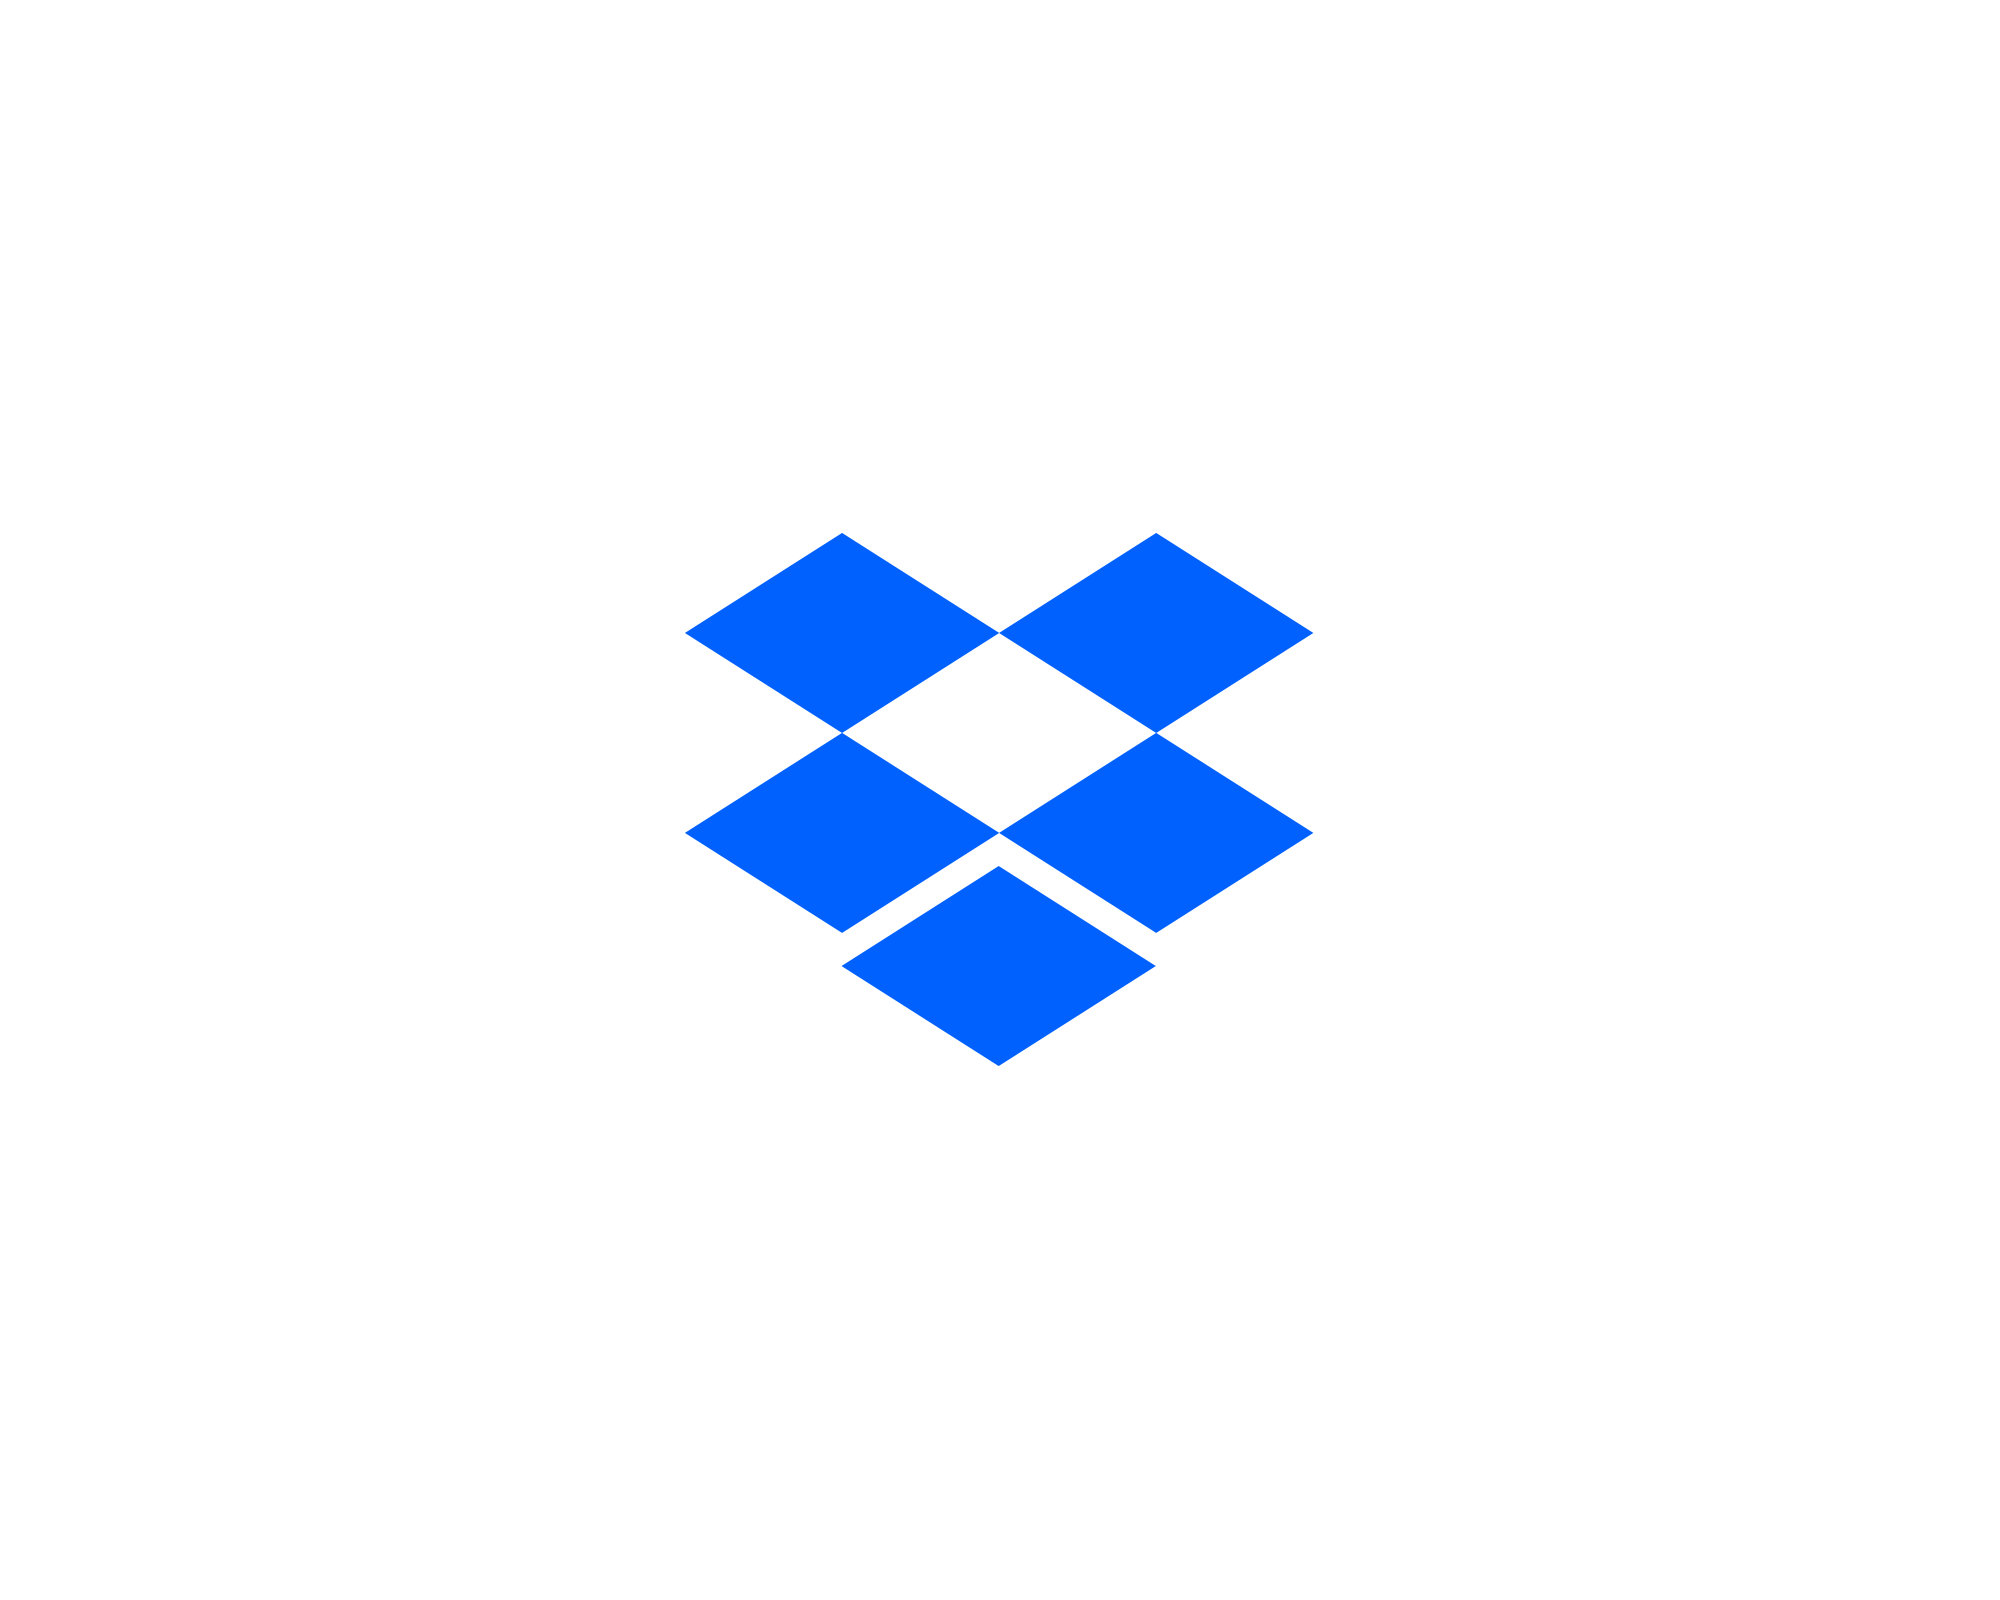
\includegraphics[scale=0.19]{logo.png}
 
%----------------------------------------------------------------------------------------
%	AUTHOR SECTION
%----------------------------------------------------------------------------------------
\begin{flushleft} \large
\emph{Autores:}\\
Antonio Gámiz Delgado \\
Samuel Medina Gutiérrez \\
Laura Sánchez Parra
\end{flushleft}

% If you don't want a supervisor, uncomment the two lines below and remove the section above
%\Large \emph{Author:}\\
%John \textsc{Smith}\\[3cm] % Your name


%----------------------------------------------------------------------------------------
%	LOGO SECTION
%----------------------------------------------------------------------------------------


 
%----------------------------------------------------------------------------------------

\vfill % Fill the rest of the page with whitespace

\end{titlepage}

\tableofcontents
\newpage

\section{Introducción}

Antes de hablar de Dropbox, vamos a comentar brevemente qué es el almacenanmiento en la nube y algunas formas de implementarlo:

Cloud-Storage es un modelo de servicio en el cual los datos son mantenidos, distribuidos, administrados y puestos a la disposición de los usuarios en una red (normalmente Internet). Los usuarios normalmente pagan por este servicio según su consumo, mensualmente, es decir, si quieres tener 5GB de almacenamiento en la nube, deberás pagar esos 5GB cada mes. 
Aunque el coste por cada GigaByte ha descendido enormemente, los proveedores de cloud storage han añadido más gastos “operativos” que puede hacer esta tecnología un poco más cara. Entre, los que por ejemplo, se encuentra la seguridad, que está siempre presente y en constante mejora ya que es una de las principales preocupaciones de los usuarios.

Este sistema presenta varias ventajas, como la facilidad de acceso a los datos desde cualquier punto con conexión a Internet, desde muchos tipos de dispositivos, la facilidad de recuperación de datos y el ahorro de los costes que conlleva comprar y mantener los propios sistemas de almacenamiento.

\section{Principales Sistemas de Almacenamiento.}

Un sistema de almacenamiento consiste en habilitar uno o varios discos duros de una red local (que a su vez puede estar conectada a Internet) de manera que los datos que allí se almacenen permanezcan accesibles a todos los dispositivos que deseen utilizarlos. De esta forma el usuario dispone de un almacenamiento común con el resto de usuarios.
La cuestión se complica cuando hay que definir la forma en que los distintos tipos de almacenamiento de datos gestionan esa conexión a tu red local.

\subsection{Network Attached Storage (NAS)}

Este sistema incorpora su propio sistema de conexión y recepción de petición de acceso a los datos, eliminando a los servidores de la ecuación. Los sistemas de almacenamiento NAS se conectan directamente al router (en local, LAN) mediante TCP/IP.

\begin{itemize}
\item Ventajas: 
\item Incovenientes: 
\end{itemize}
\subsection{Storage Area Network (SAN)}


Como un NAS, SAN traspasa la responsabilidad del almacenamiento de los datos de servidores y ordenadores a dispositivos de almacenamiento dedicados. Pero a diferencia de NAS, que es un dispositivo independiente, un SAN es una red de dispositivos de almacenamientos interconectados. Ambos son accedidos a través de la red local a la que están conectados.

\begin{itemize}
\item Ventajas: pueden acceder al dispositivo todas las personas que estén conectadas a la misma red que el NAS. Seguro, ya que somos nosotros mismos quienes manipulamos los archivos.
\item Incovenientes: dificultad en la instalación, ya que esta tiene que hacerse muy bien para su correcto funcionamiento. Caro.
\end{itemize}

\subsection{Direct Access Storage (DAS)}

Son todos los dispositvos USB, discos duros, etc, que se conectan con un computador y se tiene acceso directo al almacenamiento.


Dado que Dropbox es una empresa privada, nadie sabe exactamente cómo implementan su servicio de almacenamiento, pero se cree que usan mayormente SAN.

\section{Protocolos de Almanamiento}

Una vez vistos los principales sistemas de almacenamiento, veremos los principales protocolos usados para manejar, controlar y almacenar todos estos datos correctamente.

\subsection{Small Computer Interface (SCSI)}

SCSI es el principal método de acceso a disco en el centro de datos. El acceso a disco es realizado por medio de bloques, que son la mínima unidad de información que puede ser leída o escrita en un disco. Su tamaño varía dependiendo del tipo de disco y uso (de 512 a 4096 bytes). Este protocolo permite al servidor acceder directamente a los bloques del disco sin necesidad de un sistema de archivos.

Este protocolo se usaba principalmente para mover datos en un único servidor. EL sistema operativo se encarga de escribir datos usando SCSI, que usa un controlador para coordinar los distintos dispositivos que hay conectados al cable SCSI. Debido a que el controlador se asegura de que no haya perdida de datos, ni de que dos dispositivos estén activos a la vez en el cable, ni de que los bloques lleguen en distinto orden en que fueron enviados, la pérdida de datos y la inconsistencia es prácticamente nula.

SCSI todavía es muy usado, pero debido al aumento de complejidad en los archivos y en los centros de datos, ha sido encapsulado en el resto de protocolos.

\subsection{Fiber Channel (FC)}

El FC fue diseñado para extender la funcionalidad del protocolo SCSI en las topologías de switches y punto a punto. Esto permite conectar servidores a distancias más largas además de mejorar el consolidamiento del almacenamiento.

FC encapsula datos del protocolo SCSI y Command Descriptor Blocks (CDB) en "cargas de trabajo" del canal de fibra. Una vez encapsulados, las redes FC se encarga del direccionamiento, enrutamiento y del control de flujo requerido para soportar SCSI. Esto lo consigue asegurando la no pérdida de información en el proceso ("lossless").

Las redes FC normalmente están implementadas sobre cables de fibra óptica, con infraestructuras dedicadas. Debido a esto, proporcionan un gran ancho de banda así como una baja latencia.

\subsection{internet/IP Small Computer System Interface (iSCSI)}

iSCSI coge los datos del SCSI y los CDM y los encapsula en paquetes TCP/IP. Esto permite al protocolo SCSI ser extendido a través de las infraestructuras IP existentes.

La principal atracción de iSCSI es que el almacenamiento de datos puede ser fácilmente extendido entre la infraestructura existente con un coste adicional mínimo. Aún así, no ha conseguido ganar el mercado debido a las limitaciones del protocolo y las limitaciones de las redes tradicionales de los Data Center basadas en Ethernet.

El problema con Ethernet era que la mayoría de los data centers usaban links de 1GE que se saturaban rápidamente. Esto significaba que implementar iSCSI requería una infraestructura nueva de swicthing. 10GE ha aumentado el ancho de banda significativamente, pero no ha sido suficiente para subir la popularidad de iSCSI.

Por otro lado, como protocolo, su principal problema es que encapsula al protocolo SCSI, el cual espera la no pérdida de paquetes, llegada en el mismo orden en el que fueron enviados. Cumplir estas condiciones, usando paquetes TCP/IP que están diseñados para sufrir pérdida de paquetes y la llegada en distinto orden de los mismo, lo hace bastante complejo.

\subsection{Fiber Channel over Ethernet (FCoE)}

Protocol que se encarga de proveer la funcionalidad necesaria para ejecutar el protocolo FC sobre una red Ethernet (10GE). FCoE encapsula los paquetes del protocolo FC en paquetes Ethernet Jumbo, que aseguran que el paquete no es ni fragmentado ni alterado.


\section{Dropbox}

\subsection{Origen}
Dropbox es un servicio de almacenamiento en la nube, creado por Drew Houston y Arash Ferdows en junio de 2007. A modo de dato curioso: la idea de Dropbox se le ocurrió a Drew Houston, cuando estaba montado en un autobús de Boston a New York. En ese trayecto, él quería trabajar sobre algunas ideas de proyectos, pero se olvidó el pen drive en casa, cómo usualmente le pasaba. Así que decidió que esa sería la última vez que le pasaría, por lo que en dos demanas desarolló un prototipo y un nombre, y se lo presentó a una empresa de Silicon Valley, Y Combinator, quién invirtió en el proyecto, pero con la condición de que Houston buscara un socio, Arash Ferdows, quien estaba estudiendo ingeniería eléctrica e informática en el MIT, dejando los estudios para trabajar en lo que sería Dropbox.

\subsection{¿Qué es Dropbox?}
Dropbox se define a si mismo como una CDN (Content Delivery Network), es decir, un conjunto de servidores que contienen copias de una misma serie de contenidos (imágenes, vídeos, documentos, etc) y que están ubicados en puntos diversos de una red para poder servir sus contenidos de manera más eficiente. Normalmente usan protocolos TCP/IP y TLS que reducen la latencia.
\subsection{Edge Network}
Para facilitar al usuario una mejor experiencia, se emplean protocolos TCP/IP y TLS más cercanos a los usuarios, ya que reducen la latencia, es decir, los retardos. Dropbox está formado por una serie de PoPs (Points of Presence) situados estratégicamente alrededor del mundo para reducir los tiempos de retardo.

Por lo que, la Edge Network de Dropbox es, el conjunto de PoPs que permiten reducir los tiempos de latencia.

\subsection{GSLB - Global Server Load Balancing}

¿Cómo distribuye Dropbox los usuarios entre los Pops? Utiliza GSLB, normalmente GSLB envía cada usuario al Pop más cercano, a no ser que el Pop esté inhabilitado.

\subsubsection{BGP anycast}
Anycast es el método más fácil de loadbalancing. Usa el protocolo de routing del núcleo de Internet, BGP (Border Gateway Protocol - protocolo meidente el cuál se intercambia información de encaminamiento entre sistemas autónomos). Para empezar a usar anycast es suficiente con empezar a "publicar" la misma subred desde todos los PoPs e Internet entregerá cada paquete al PoP "óptimo" automáticamente. Aunque parece ser un muy buen método, tiene varias desventajas, como el limitado control que se tiene sobre el tráfico y es difícil mover tráfico implícitamente de un PoP a otro.

BGP anycast en Dropbox: debido a sus desventajas, sólo se usa para los dominos APEX, como dropbox.com (sin www) y como "último recurso" en caso de un ataque DDoS.

\subsubsection{GeoDNS}
En este método cada PoP tiene su propio y único espacio de direcciones IP y DNS es el responsable de asignar a IP diferente a cada usuario basado en su localización geográfica. Esto nos da más control sobre la dirección del tráfico, además, la configuración es más fácil y la solución de problemas es más simple.

GeoDNS en Dropbox: En este momento, están trabajando con el enrutamiento basado en LatLong (coordenadas geográficas), que es relativamente complejo.

\subsubsection{Hybrid unicast/anycast GSLB}

Combinación de las dos anteriores, que permite beneficiarse de las ventajas de los dos métodos.

\subsubsection{Real User Metrics}
Los métodos anteriores tienen un problema: ninguno de ellos usa datos de performance (actuación) percibido por los usuarios, sino que dependen en aproximaciones. Para arreglar eso, RUM usa datos de de las performances de los clientes de escritorio.

RUM en Dropbox: todavía es un proyecto en evolución que todavía no está implementado para el público general, pero se están realizando experimentos y recogiendo datos de los métodos anteriores para poder llegar a usar hasta 25-30 PoPs.

\subsection{Backbone Network}
Junto con la edge network, Dropbox ha creado una backbone network que permite la interconexión entre los data centers de Norte América no sólo entre ellos, sino también con los nodos edge alrededor del mundo.

A nivel interno (IGP)(Conexión entre PoPs); 
Dropbox gestiona interfaces en múltiples redes cuya tarea es copiar paquetes de una red a otra en función de las tablas de enrutamiento almacenadas en la memoria.

La arquitectura de enrutamiento es  Open Shortest Path First (OSPF) que usa el algoritmo Dijkstra, para calcular la ruta más corta entre dos nodos.

Actualmente Dropbox utiliza IPv6, una versión del Internet Protocol (IP), definida en el RFC 2460.

A nivel externo (BGP)(Conexión con otros edge nodos); se tienen en cuenta dos diseños básicos. 
\begin{enumerate}
\item Diseño BGP de malla completa en todos los routers, es decir, todos los routers conocen todas las rutas entre sí. Esto funciona bien en una red más pequeña.

\item División de la red troncal en regiones más pequeñas. Al mismo tiempo que implementar BGP de malla completa entre los routers dentro de una misma región, mientras que los RR anuncian rutas entre las regiones.
Los RR o route reflector son dispositivos que permiten la conexión entre dos routers sin necesidad de una malla completa, es decir, un router se conecta con el RR y este a su vez la refleja en otro router.


\subsection{Tipos de routers}
La red troncal de Dropbox consta de routers con tres funciones distintas:
\begin{itemize}
\item Routers del centro de datos (DR): con una función principal de conectar el centro de datos a la red troncal.
\item Routers de red troncal (BB): que actúan como un punto de terminación para circuitos de larga distancia y también como dispositivos de agregación para DR en regiones donde tenemos centros de datos.
\item Peering routers (PR): con una función principal de conectar Dropbox a pares BGP externos para proporcionar conectividad a Internet

\end{itemize}



\section{Dropbox LAN Sync}

Para terminar, vamos a hablar de una de las nuevas funciones de Dropbox, Dropbox LAN Sync:


Dropbox Lan Sync es un tecnología que permite descargar archivos desde otras computadoras que estén conectadas a tu misma red, sin la necesidad de conectar a los servidores de Dropbpox, ahorrando así tiempo y ancho de banda. Cualquier ordenador que esté conectado a la misma red, podrá acceder al resto y descargar el archivo directamente desde allí.
Para comprender el funcionamiento de esta tecnología, debemos conocer las abstracciones que usa DropBox: Los bloques y los espacios de nombres. 
\begin{itemize}
	\item Bloques: los archivos en DropBox están separados en bloques de 4MB direccionados por funciones HASH. Por tanto un archivo puede ser descrito por una lista de “Hashes”.
	\item Espacios de nombres:   pueden ser pensados como directorios con permisos específicos. Cada cuenta tiene un espacio de nombre que representa su cuenta personal  y todos los archivos que contiene. 
\end{itemize}



La petición de descargas de archivos puede pensarse como una serie de peticiones de pares (espacio de nombres, Hashes) para indicar  la computadora y el/los bloques específicos . Sin LAN Sync estas peticiones se meterían en una cola  y enviadas al servidor de bloques que devuelve un bloque de datos. Por tanto, no es necesario que la tubería de descarga conozca cosas como el nombre del archivo. ¿Qué significa esto? Que  LAN SYNC solo sincroniza los datos reales de los archivos, ya que los metadatos los proveen los servidores de DropBox. De esta forma se tiene la certeza de que todos los computadores y archivos estarán siempre en un estado consistente.


En definitiva, nos encontramos con una red P2P, en la cual primero intentaremos descargar el archivo desde los peers ubicados en la red, usando el servidor de bloques solamente si esta última acción falla.

Esta tecnología tiene tres componentes principales:
\begin{itemize}
\item El “Discovery engine” que trata de encontrar máquinas que estén conectadas en la red que se puedan sincronizar. Para hacer esto cada máquina envía y escucha periódicamente de paquetes UDP sobre el puerto 17500. Estos paquetes contienen información sobre el protocolo usado, el espacio de nombres soportado…
\item Protocolo:  la transferencia del bloque se hace mediante HTTPS. Cada computadora tiene que poner en marchaun servidor HTTPS. Este soporta dos métodos, GET y HEAD. El método HEAD se usa para comprobar si el bloque existe y GET devuelve el bloque.
\item Servidor/Cliente: el servidor maneja peticiones de los clientes conectados en el servidor, proveyendo los bloques de datos solicitados. Los clientes solo son responsables de realizar las peticiones.  
\end{itemize}
\end{enumerate}
\newpage
\begin{thebibliography}{9}
\bibitem{nombre} https://blogs.dropbox.com/tech/2017/06/evolution-of-dropboxs-edge-network/
\bibitem{} https://computerhoy.com/noticias/internet/que-es-como-funciona-almacenamiento-red-33081 
\bibitem{} https://blogs.dropbox.com/tech/2017/09/infrastructure-update-evolution-of-the-dropbox-backbone-network/
\bibitem{} https://blogs.dropbox.com/tech/2016/05/inside-the-magic-pocket/
\bibitem{} https://blogs.dropbox.com/tech/
\bibitem{} https://blogs.dropbox.com/developers/
\bibitem{} https://blogs.dropbox.com/tech/2015/10/inside-lan-sync/
\bibitem{}  https://www.makeuseof.com/tag/network-storage-explained-cloud-nas-san-das/
\end{thebibliography}

\end{document}